\documentclass[runningheads]{llncs}
\usepackage[T1]{fontenc}
\usepackage[utf8]{inputenc}
\usepackage{graphicx}
\usepackage{booktabs}
\usepackage{amsmath,amssymb}
\usepackage{microtype}
\usepackage{array}
\usepackage{url}
\usepackage[hidelinks]{hyperref}
\providecommand{\tightlist}{\setlength{\itemsep}{0pt}\setlength{\parskip}{0pt}}
\setlength{\tabcolsep}{4pt}
\renewcommand{\arraystretch}{0.95}

\begin{document}

\title{Reasoning Under Context Competition: A Controlled Study of Coordination Overhead in LLM Calls}
\titlerunning{Reasoning Under Context Competition}
\author{Anonymous Authors}
\authorrunning{Anonymous Authors}
\institute{Anonymous Institution}
\maketitle

\begin{abstract}
Multi-agent and memory-augmented LLM systems often place coordination content, such as shared state, prior discussion, or intermediate summaries, into the same finite context window used for the task itself, creating direct competition between coordination tokens and task-relevant reasoning tokens. We study this tradeoff with the Roundtable Context Window Test (RCWT), a controlled protocol that varies coordination overhead while holding total context budget fixed. Across three commercial models on a context-dependent recall task, performance remains strong through moderate overhead and then degrades sharply at extreme overhead levels; among several simple candidate families, a logistic curve provides the best empirical fit to the observed transition. At a 4,096-token budget, the degradation region appears near 91--94\% coordination overhead, although the exact location and steepness are model- and task-dependent. Additional experiments at larger context budgets suggest that this behavior may be better explained by a minimum remaining task-execution context reserve than by a fixed coordination proportion alone, but we view this as a preliminary interpretation that requires validation across additional window sizes and task families. We further find substantial task dependence: self-contained algorithmic tasks show little degradation, contradictory coordination content produces a distinct distraction pattern in one model family, and pack-style DROP probes require a much larger residual task budget than compact reasoning probes. Overall, RCWT provides a controlled methodology for studying context competition in LLM calls and suggests that practical systems should explicitly reserve task-specific execution budget rather than treating coordination context as cost-free.
An anonymized replication package is available at \url{https://anonymous.4open.science/r/rcwt-artifact-3DD8/}.
\keywords{Large language models \and Multi-agent systems \and Context windows \and Reasoning \and Benchmarking}
\end{abstract}

\section{Introduction}\label{introduction}

Multi-agent and memory-augmented LLM systems increasingly assemble multiple functional components inside a single model context: agent messages, retrieved memories or documents, summaries of prior context, tool observations, and coordination instructions \cite{ram-etal-2023-context,toolformer,autogen,guo2024multiagents}. This composition is constrained by predefined context-window limits, which can become binding in settings such as extended conversations, document summarization, and long-horizon reasoning \cite{longlora}. We study the per-call version of this problem, not full session-level multi-agent dynamics. A single call may contain the task, retrieved memories, summaries of prior turns, intermediate conclusions from other agents, tool outputs, and instructions for how the current model should coordinate with the rest of the system. These components are operationally useful, but they occupy the same finite context window. This motivates studying how task performance changes as non-task coordination content consumes more of the available input budget, especially given evidence that LLMs do not always use long contexts robustly \cite{lostmiddle,du2025contextlength}.

This paper studies a narrow version of that competition: in a single LLM call with fixed context budget \(W\), what happens as coordination content \(c\) increases and the remaining task block \(W-c\) shrinks? For convenience, we refer to this fixed-budget tradeoff as \emph{context competition}. For a model \(M\), we define \(R_M(c,W,T)\) as the expected response quality on task family \(T\) when \(c\) tokens of the context window are occupied by coordination content under total budget \(W\). In our experiments, \(R_M\) is estimated empirically using task-specific performance metrics such as accuracy. Thus, our object of study is not a universal property of LLMs, but a family of model- and task-dependent response quality curves.

We introduce the Roundtable Context Window Test (RCWT), a controlled protocol that varies coordination overhead while holding total context budget fixed. RCWT is designed to isolate coordination-token pressure from other multi-agent confounds such as turn scheduling, tool failures, memory retrieval policy, and agent topology. The protocol measures a single model call at a time, with fixed task content, fixed coordination content, explicit position control, and binary scoring against precomputed ground truth.

Our central empirical finding is intentionally scoped. On a context-dependent technical-specification recall task across three commercial models, quality remains high through moderate coordination overhead and then degrades sharply at extreme overhead. A logistic curve best summarizes the observed transition among the simple candidate families tested. At \(W=4096\), the transition appears near 91--94\% coordination overhead. Additional window-size experiments suggest that the transition is better described by a minimum remaining task budget than by a fixed overhead proportion alone, but this interpretation should be treated as exploratory and task-dependent.

The paper makes four contributions:

\begin{enumerate}
\def\labelenumi{\arabic{enumi}.}
\tightlist
\item
  \textbf{A controlled methodology.} RCWT varies coordination proportion with fixed context budget, position control, binary scoring, and multi-provider evaluation.
\item
  \textbf{An empirical characterization.} On the main context-dependent task, all three tested providers show a sharp high-overhead degradation pattern; a logistic curve is the best empirical fit among five simple candidate forms.
\item
  \textbf{A task-dependence analysis.} Self-contained algorithmic tasks do not show the same degradation, while contradictory coordination content produces a distinct model-dependent distraction pattern.
\item
  \textbf{A practical implication.} Coordination content should be budgeted explicitly. For systems operating in task regimes similar to the main RCWT task, preserving a calibrated task-specific residual budget is safer than relying on a fixed coordination proportion.
\end{enumerate}

The claim is not that RCWT discovers a universal context law. The claim is that RCWT gives a reproducible way to measure how task quality changes when coordination content competes with task content inside one LLM call.

\section{Related Work}\label{related-work}

\textbf{Long-context behavior.} Prior work shows that larger context windows do not guarantee uniform use of all positions. The ``lost in the middle'' result demonstrates that LLMs can underuse relevant information placed away from the beginning or end of a long context \cite{lostmiddle}. LongBench broadens long-context evaluation across single-document QA, multi-document QA, summarization, few-shot learning, synthetic tasks, and code completion \cite{longbench}. RULER further expands needle-in-a-haystack style testing with configurable sequence length and task complexity, including multi-hop tracing, aggregation, and QA-style tasks \cite{ruler}. RCWT asks a different but adjacent question: not only where relevant content is placed or how far a model's effective context extends, but how quality changes when coordination content consumes increasing fractions of a fixed per-call window.

\textbf{Attention and systems bottlenecks.} Long-context systems face computational and memory pressure from attention and KV-cache growth. Long-context extension methods also show that expanding usable context often requires architectural, training, or attention-pattern changes rather than merely increasing a nominal token limit \cite{longlora}. Efficient-attention work reduces these costs through IO-aware exact attention or sparse/local/global attention patterns \cite{flashattention,longformer,bigbird}. These methods address how to make long contexts feasible; RCWT measures whether the feasible context is being allocated to coordination or to the task content needed by the current call.

\textbf{Context compression.} Prompt and context compression methods such as LLMLingua-2 reduce token count while attempting to preserve task-relevant information \cite{llmlingua2}. RCWT can be viewed as a complementary measurement tool: if compression reduces coordination tokens without destroying relevant state, it should move a call away from the high-overhead transition region.

\textbf{Multi-agent coordination overhead.} LLM multi-agent systems introduce coordination costs through inter-agent communication, role specification, orchestration, and task verification \cite{mast}. Recent scaling studies further show that adding agents can yield diminishing or negative returns when coordination overhead, error amplification, or task structure dominate the benefits of parallelism \cite{scalingagents}. However, such systems usually combine several mechanisms at once, including decomposition, debate, voting, tool use, memory, and orchestration. RCWT isolates one component: competition between coordination tokens and task tokens in a single call.

\textbf{External benchmark probes.} GSM8K evaluates grade-school mathematical reasoning \cite{gsm8k}; MMLU-Pro evaluates robust multi-task language understanding \cite{mmlupro}; and DROP evaluates discrete reasoning over paragraphs \cite{drop}. We do not use these as leaderboard benchmarks. Instead, we adapt them into pack-style RCWT stress probes to check whether high-overhead behavior appears outside the original technical-specification task. We do not run RULER in this submission because RULER primarily varies effective sequence length and task complexity, whereas RCWT fixes \(W\) and varies the coordination/task allocation inside a single call. A RULER-style RCWT variant is a natural follow-up.

\section{Method}\label{method}

\subsection{Problem Setup}\label{problem-setup}

Let \(W\) be a fixed context budget. Let \(c\) be the number of tokens allocated to coordination content, and let \(p=c/W\) be the coordination proportion. The remaining budget \(W-c\) is allocated to task content. RCWT estimates a quality function:

\[
R_M(c,W,T) \in [0,1],
\]

where \(T\) denotes the task family. Quality is measured against binary ground truth or exact answer extraction, depending on the task.

\subsection{RCWT Protocol}\label{rcwt-protocol}

The main RCWT task is context-dependent recall over a technical software specification. The coordination block is synthetic but structured: it follows a multi-agent/Roundtable context format with role and protocol descriptions, inter-agent message history, shared state and propositions, and tool schemas. We do not use real production logs in the central tests; Task 4 uses a Roundtable-style transcript that is likewise controlled and constructed to admit clean ground truth. The correct characterization is therefore realistic controlled coordination content, not real Roundtable logs. The task block asks for a structured response whose scored facts must be recovered from that document. This design is related to long-context retrieval and recall evaluations, including key-value retrieval and needle-in-a-haystack style probes, but differs in that RCWT varies the fraction of the fixed context budget consumed by coordination content rather than only varying context length or answer position \cite{lostmiddle,ivgi-etal-2023-efficient}. Two items absent from the reference specification are excluded from the effective score, yielding an 8-item effective score. For example, a scored item may check whether a named configuration option is enabled, deprecated, or subject to a stated constraint in the preceding specification. See Appendix A for a representative example.
The main experiment uses \(W=4096\) and coordination proportions \(p \in \{0, 25, 50, 75, 90, 92, 94, 96, 98\}\%\). Each cell is run in two position orders: \texttt{coord\_first}, where coordination content precedes the task, and \texttt{reason\_first}, where the task precedes coordination content. This order control is motivated by prior evidence that LLM performance can depend strongly on where relevant information appears within a long context \cite{lostmiddle}. The primary \(W=4096\) suite uses \(N=20\) trials per cell.

The sample size is cost-bounded but targeted at large effects. Pooling both orders gives 40 calls and 320 binary item observations per proportion on the main 8-item effective score. We report Wilson 95\% confidence intervals for binomial proportions \cite{wilson1927probable} and two-proportion tests for the main baseline-vs-high-overhead comparison. This design is adequate for the observed 15--34 percentage-point drops at 90\% overhead, but not for small-effect claims; those remain exploratory.

\subsection{Candidate Curves}\label{candidate-curves}

For the main context-dependent task, we fit five simple candidate families: logistic, power law, exponential, quadratic, and piecewise linear. These families were chosen as descriptive baselines spanning plausible degradation shapes: a bounded S-shaped threshold, gradual exponential decay, heavy-tailed power-law decay, smooth polynomial curvature, and an explicit breakpoint model. They are not treated as mechanistic proofs. The logistic form is:

\[
R_M(c,W,T)=\frac{R_0}{1+\exp(k(c/W-p_0))},
\]

where \(R_0\) is the baseline score, \(p_0\) is the fitted transition location, and \(k\) controls transition steepness. We treat this as an empirical summary, not a mechanistic derivation.

\subsection{Boundary Tasks}\label{boundary-tasks}

To test whether coordination overhead alone explains degradation, RCWT includes boundary tasks:

\begin{itemize}
\item
  \textbf{Self-contained algorithmic task.} The task block contains a Python function, one concrete input, and ten yes/no questions about the execution trace. The correct answers can be computed entirely from the task block; the coordination block is intentionally irrelevant. If performance remains stable as coordination grows, this indicates that overhead is not harmful merely because it adds unrelated text. See Appendix A for a representative example.
\item
  \textbf{Context-distraction task.} The task block asks yes/no questions about general data-engineering and product-practice priors. The coordination block is a meeting transcript with salient project-specific decisions that sometimes conflict with those priors, such as choosing an in-house masking layer because a vendor failed a System and Organization Controls (SOC) 2 requirement. This probes semantic distraction: coordination content may hurt by changing which evidence the model treats as salient, not only by consuming tokens. See Appendix A for a representative example.
\item
  \textbf{External benchmark probes.} We adapt GSM8K, MMLU-Pro, and DROP into \emph{pack-style} RCWT probes by grouping 10 benchmark items into a single model call. Each pack preserves the original task format at the item level, but the larger combined task block makes coordination overhead materially affect the residual task budget. This design avoids treating isolated one-question prompts as meaningful stress tests of context competition, since such prompts are often too small for high-overhead truncation to affect the task content.
\end{itemize}

\subsection{Models and Setup}\label{models-and-setup}

Three commercial models from different providers are tested: Gemini 2.0 Flash, Claude Haiku 4.5, and GPT-4.1-mini. Calls use direct provider APIs rather than a multi-agent framework, because the goal is to isolate the single-call context competition effect.

For double-anonymous review, the replication package is prepared as an anonymized source artifact containing experiment scripts, prompt templates, result summaries, and plotting code. The public repository link will be added after the review process permits deanonymization.

\section{Results}\label{results}

\subsection{Main Context-Dependent Task}\label{main-context-dependent-task}

Table 1 shows the pooled main-task scores at \(W=4096\). All three models maintain high scores at low and moderate coordination overhead. Degradation becomes sharp in the 90--98\% region.

\begin{table}[t]
\centering
\small
\caption{Main context-dependent RCWT task at $W=4096$, pooled over position order. Scores are effective binary accuracy.}
\begin{tabular}{lrrrr}
\toprule
Coord. overhead & Task tokens & Gemini & Haiku & GPT \\
\midrule
0\%  & 4096 & 1.000 & 0.972 & 1.000 \\
25\% & 3072 & 0.960 & 0.906 & 0.972 \\
50\% & 2048 & 0.944 & 0.894 & 0.988 \\
75\% & 1024 & 0.894 & 0.875 & 0.981 \\
90\% & 410  & 0.659 & 0.666 & 0.853 \\
92\% & 328  & 0.404 & 0.456 & 0.600 \\
94\% & 246  & 0.012 & 0.119 & 0.406 \\
96\% & 164  & 0.012 & 0.088 & 0.319 \\
98\% & 82   & 0.000 & 0.050 & 0.337 \\
\bottomrule
\end{tabular}
\end{table}

At 90\% overhead, degradation from baseline is 34.1 percentage points for Gemini, 30.6 points for Haiku, and 14.7 points for GPT. The GPT curve is shallower, but not flat: it also degrades significantly in the high-overhead region.

\begin{figure}[t]
\centering
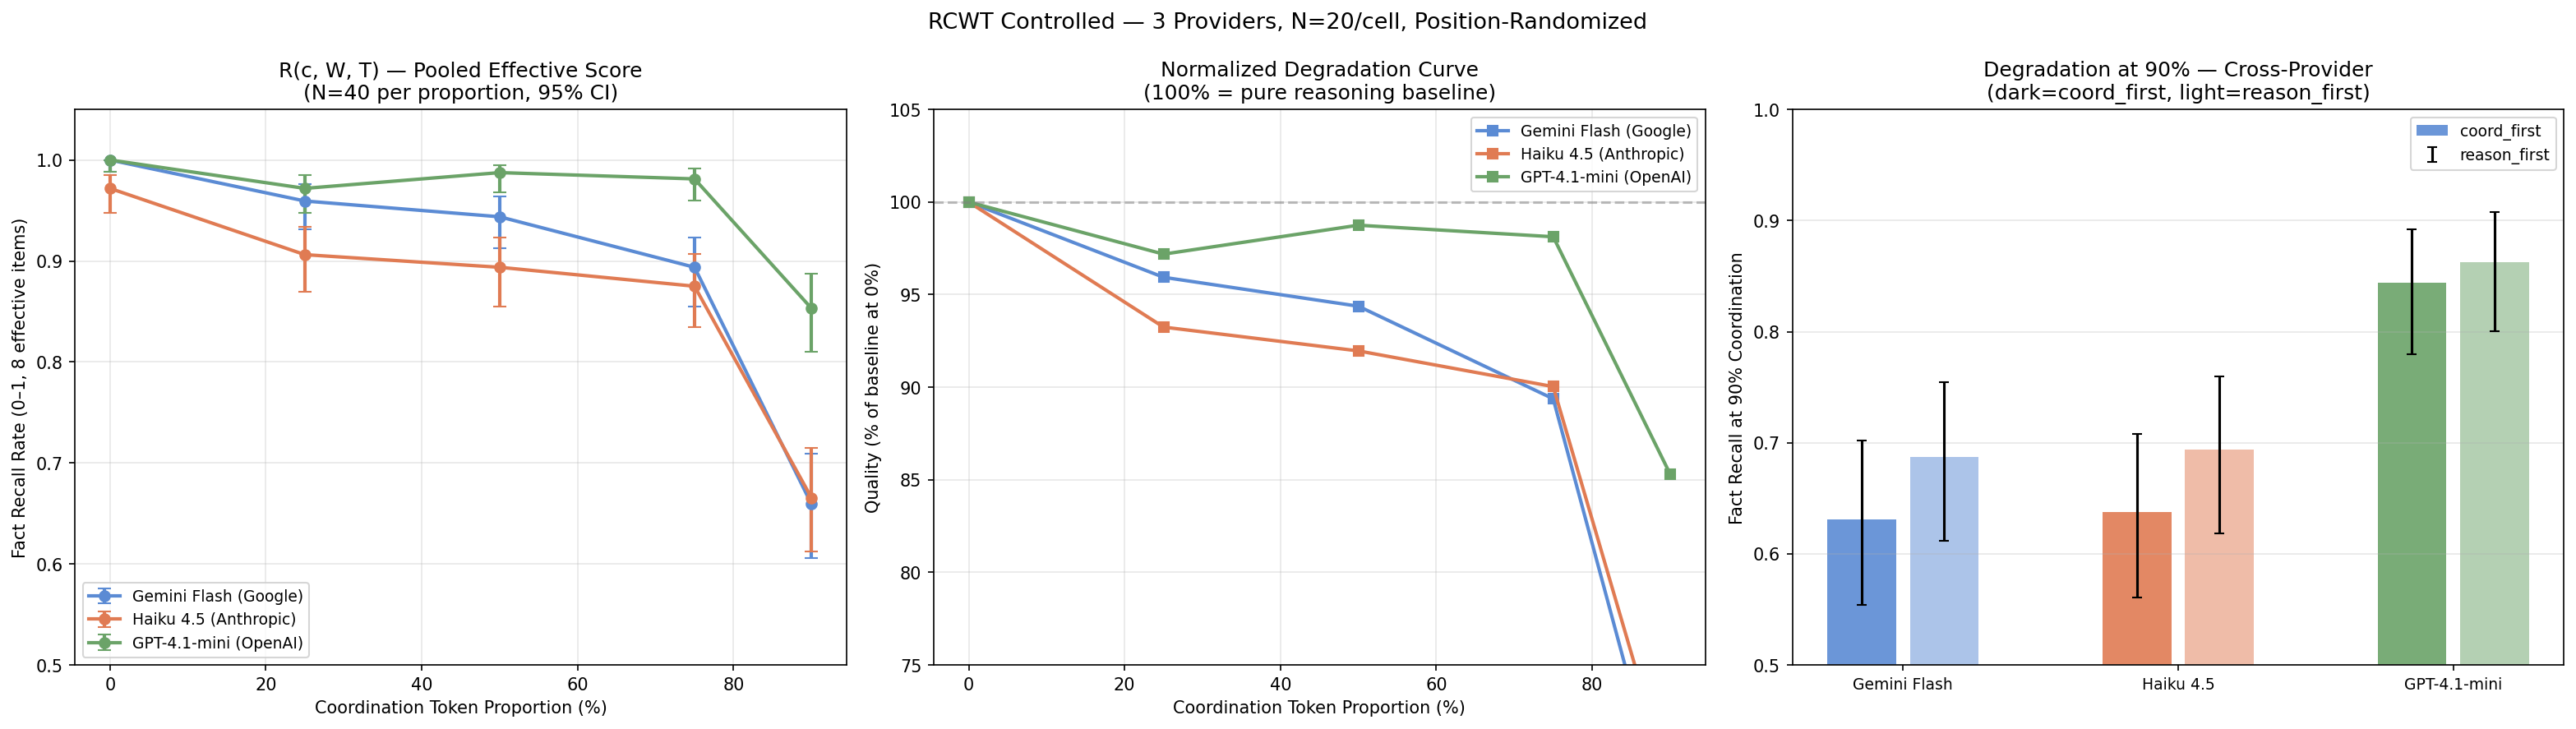
\includegraphics[width=0.95\linewidth]{figures/rcwt_cross_provider.png}
\caption{Cross-provider RCWT scores on the main context-dependent task. The transition appears only at high coordination overhead for this task and budget.}
\end{figure}

Table 2 summarizes the statistical comparison and fitted transition. Logistic decay has the best AIC among the tested candidate families and high \(R^2\) for all three providers. The fitted transition region is model-dependent but lies within a narrow range for this task at \(W=4096\). The AIC comparison is descriptive model selection over nine sampled proportions, not evidence that the logistic family is a universal law.

\begin{table}[t]
\centering
\scriptsize
\caption{Main-task statistical and fit summary at $W=4096$. Accuracy CIs are Wilson 95\% intervals over 320 item-level observations per pooled proportion. $p$-values are two-proportion z-tests comparing 0\% and 90\% overhead. AIC reports logistic vs. next-best family.}
\resizebox{\linewidth}{!}{%
\begin{tabular}{lccccccc}
\toprule
Model & 0\% acc. [CI] & 90\% acc. [CI] & $\Delta$ pp & $p$ & $p_0$ & $R^2$ & AIC log./next \\
\midrule
Gemini 2.0 Flash & 1.000 [0.988,1.000] & 0.659 [0.606,0.709] & -34.1 & $<10^{-12}$ & 0.913 & 0.988 & -24.2 / 0.5 \\
Claude Haiku 4.5 & 0.972 [0.947,0.985] & 0.666 [0.612,0.715] & -30.6 & $<10^{-12}$ & 0.917 & 0.990 & -27.8 / -1.9 \\
GPT-4.1-mini & 1.000 [0.988,1.000] & 0.853 [0.810,0.888] & -14.7 & $<10^{-12}$ & 0.939 & 0.957 & -19.5 / -6.3 \\
\bottomrule
\end{tabular}%
}
\end{table}

These results show that nominal context-window size and average prompt length are incomplete safety signals. In this task family, performance can remain stable while coordination content grows through most of the window, then change rapidly once the residual task budget enters the high-overhead region.

\subsection{Window Scaling}\label{window-scaling}

A fixed-proportion explanation would predict that 90\% overhead should have similar effects at different context budgets. The observed pattern does not match that simple account. At \(W=4096\), 90\% overhead leaves about 410 task tokens and falls near the degradation region. At \(W=8192\), the same 90\% overhead leaves about 819 task tokens and produces much smaller degradation.

We model this with a task-specific residual budget parameter \(\theta\). In this interpretation, the transition location follows:

\[
p_0(W)=1-\frac{\theta}{W}.
\]

The point is not that \(\theta\) is universal; it is an empirical estimate for a given task/model pair. Table 3 summarizes the observed fit across three window sizes for the main task.

\begin{table}[t]
\centering
\small
\caption{Window-scaling summary for the main task. Prediction uses $\theta$ estimated from the $W=4096$ fit.}
\begin{tabular}{lrrrr}
\toprule
Model & $\theta$ & Pred. $p_0$(8K) & Obs. $p_0$(8K) & Obs. $p_0$(16K) \\
\midrule
Gemini 2.0 Flash & 356 & 95.7\% & 96.0\% & 97.9\% \\
Claude Haiku 4.5 & 340 & 95.8\% & 96.2\% & 98.1\% \\
GPT-4.1-mini & 250 & 96.9\% & 97.1\% & 98.4\% \\
\bottomrule
\end{tabular}
\end{table}

Across the \(4K\), \(8K\), and \(16K\) runs, the maximum transition-location error is 0.37 percentage points. This is strong evidence that the fixed-proportion story is incomplete for the main task. However, the interpretation remains bounded: different tasks can have different \(\theta\) values, and architectural behavior at much larger windows may differ.

A \(W=32768\) extension further supports the direction of the pattern. At that budget, 97.5\% overhead leaves about 819 task tokens, and the strongest degradation appears only at 99\% overhead, where the remaining task budget is about 328 tokens. The Gemini row in this extension uses Gemini 2.5 Flash rather than Gemini 2.0 Flash, so the \(32K\) experiment is treated as extension evidence rather than a direct continuation of the original three-model scaling series.

\subsection{Task Dependence}\label{task-dependence}

RCWT is intended to characterize task regimes, not only model identities. The boundary tasks show that coordination overhead does not have a single universal effect.

\subsubsection{Self-Contained Algorithmic Task}\label{self-contained-algorithmic-task}

In the self-contained algorithmic task, the relevant information is in the task block itself. The coordination content is irrelevant. All three providers maintain performance across the tested overhead levels. This suggests that the high-overhead effect in the main task is not caused merely by longer prompts or by the presence of irrelevant text. It appears when coordination content displaces information needed for the task. The aggregate evidence for this boundary task is in \texttt{results/task2/}.

\subsubsection{Context-Distraction Task}\label{context-distraction-task}

The context-distraction task creates a different failure mode. The coordination content contains salient claims that conflict with the correct answers. Haiku is the only tested model that degrades strongly in this setup: its pooled score falls from 0.888 at 0\% overhead to 0.670 at 25\% and 0.410 at 50\%, while GPT remains near 0.88--0.92 and Gemini remains at 0.900. The order split is large for Haiku, so we present this as model-specific exploratory evidence rather than a general law. Detailed aggregate files are included in the supplementary materials; representative prompt fragments appear in Appendix A. This pattern indicates that coordination content can hurt not only by consuming budget, but also by changing which evidence a model treats as salient.

\subsection{Cross-Benchmark Generalization}\label{cross-benchmark-generalization}

The first one-question GSM8K and MMLU-Pro probes were underpowered for RCWT: their task blocks were short enough that little meaningful truncation occurred at 90\% overhead. We therefore use 10-item packs per call and add DROP as a passage-heavy reading-comprehension probe. Table 4 reports the corrected pack probes.

\begin{table}[t]
\centering
\small
\caption{Task-dependent residual budget estimates at $W=4096$. Pack probes are RCWT stress probes, not leaderboard estimates.}
\begin{tabular}{lrrl}
\toprule
Probe & Fitted $p_0$ range & Approx. reserve & Truncation onset \\
\midrule
Task 1 spec recall & 0.913--0.939 & 250--356 tok & main task \\
GSM8K-pack & 0.853--0.893 & 438--602 tok & 90\% \\
MMLU-Pro-pack & 0.733--0.755 & 1003--1094 tok & 50\% partial \\
DROP-pack & 0.481--0.624 & 1539--2126 tok & 50\% \\
\bottomrule
\end{tabular}
\end{table}

The pack probes are consistent with the RCWT pattern: performance remains near baseline while the full task block fits, then drops when the task block is truncated. The transition location differs by benchmark: DROP shifts earlier because the passage-heavy task block truncates by 50\% overhead. These \(p_0\) values are descriptive interpolations over five sampled proportions, not evidence of a universal logistic law. The results should not be cited as model benchmark performance because the prompt format asks for multiple compact answers in one call.

\section{Discussion}\label{discussion}

\subsection{Implications}\label{implications}

The main engineering implication is simple: coordination context is not free. Prior work on long-context language models shows that performance can degrade as relevant information is displaced within long inputs, and prompt-compression work treats context length as an explicit cost to be managed \cite{lostmiddle,jiang-etal-2023-llmlingua}. Systems that append agent history, retrieved memories, intermediate summaries, and shared state should therefore track the resulting coordination proportion and the residual task budget.

For tasks similar to the main RCWT task, a conservative heuristic is to reserve a few hundred tokens for the task block; the fitted value is roughly 400 tokens at the tested complexity level. This number is not universal; it is a calibration point. The cross-task results show why: the estimated residual budget ranges from a few hundred tokens in the main recall task to roughly 1.5K--2.1K tokens in DROP-style passage reasoning, and the DROP transition is smoother because the task block becomes partially or fully truncated earlier. The safer design pattern is to measure \(\theta\) for the task family and model, then budget coordination around that value.

Compression and state-structuring methods become useful when they preserve relevant coordination information while reducing token count \cite{jiang-etal-2023-llmlingua,llmlingua2}. The context-distraction results also suggest that structure matters: systems should distinguish factual state, inference, uncertainty, and contradiction rather than mixing them into undifferentiated transcript text. This is consistent with agent-memory systems that separate active context from longer-term or retrieved memory, and with reflection-based agents that store distilled feedback rather than raw interaction traces \cite{park2023generativeagentsinteractivesimulacra,packer2024memgptllmsoperatingsystems}.

\subsection{Threats to Validity}\label{threats-to-validity}

\textbf{Exploratory design.} The main sweep was developed iteratively: early cells suggested a flat region, and cliff cells were added afterward. The fits should be read as empirical characterization and hypothesis generation, not as pre-registered confirmation.

\textbf{Task coverage.} The main logistic result is strongest for one technical-specification recall task. Task 4 and the benchmark packs broaden coverage, but a confirmatory study should pre-register more task families. This matters because RCWT estimates a task-specific residual budget: tasks vary in whether relevant evidence is self-contained, retrieved from context, semantically contradicted by coordination content, or truncated under packing. A broader pre-registered set would separate these regimes more cleanly and reduce the risk that the main logistic pattern reflects the idiosyncrasies of one technical-specification task.
\textbf{Judge calibration.} The main task uses an automated judge for open-ended response parsing. Cross-vendor re-scoring did not show clear evidence that judges favored outputs from their own model family or provider, but judge-specific strictness remains a limitation.

\textbf{Tokenization.} Providers use different tokenizers. Post-hoc calibration using provider-reported input token counts shows that the cliff-range correction is small relative to the observed model spread, but native tokenization should be preferred in future runs.

\textbf{Single-call scope.} RCWT measures one inference call with controlled context composition. Multi-agent sessions add retrieval policies, memory summarization, turn scheduling, and tool-mediated state changes. RCWT should therefore be used as a local measurement primitive, not as a full session-level theory.

\textbf{Output length.} A possible alternative explanation is that high overhead leaves too little output space, producing shorter responses. Output-length analysis does not support this for Haiku and GPT: responses remain near baseline length while accuracy drops. Gemini shows a partial physical-budget interaction only beyond the quality transition.

\section{Conclusion}\label{conclusion}

RCWT provides a controlled way to study context competition in LLM calls. Across three commercial models on a context-dependent recall task, quality remains high through moderate overhead and then degrades sharply near extreme coordination proportions. A logistic curve is the best empirical summary among the candidate families tested, while window-scaling experiments suggest that the transition is better explained by a task-specific execution reserve than by a fixed coordination proportion alone. The result should not be read as a universal threshold of reasoning tokens. It is a measurement framework plus an empirical warning: coordination content can silently consume the task budget on which the current call depends.

\section*{Acknowledgements}

We used LLM tools to assist with grammar correction and rephrasing during manuscript preparation. The authors take full responsibility for the content, experiments, analysis, and claims.

\bibliographystyle{unsrt}
\bibliography{references}

\appendix
\renewcommand{\theHsection}{appendix.\arabic{section}}
\section{Prompt and Task Examples}\label{prompt-and-task-examples}

The experiments use controlled prompt fragments rather than production logs. Full prompt templates and aggregate files are included in the review artifact.

\textbf{Main context-dependent task.} The coordination block is a technical specification. A representative excerpt states that PostgreSQL LISTEN/NOTIFY has an 8KB payload limit, Redis Pub/Sub handles roughly 100K messages per second but has no persistence, and Redis Streams has persistence with about 5ms latency versus about 1ms for Pub/Sub. The model is asked for a structured technical analysis, and binary scored items check whether these facts are recovered correctly.

\textbf{Self-contained algorithmic task.} The task block gives a Python function that partitions \texttt{items={[}3,\ 10,\ 15,\ 7,\ 10,\ 22,\ 4{]}} around \texttt{threshold=10}. Representative scored questions ask whether the sum is 71, whether indices 2 and 5 are above threshold, and whether the maximum above-threshold value is 22. The answers are fully determined by the code and input, so the coordination block is irrelevant.

\textbf{Context-distraction task.} The coordination block is a controlled meeting transcript for an invented data-platform project. It states that Kafka Streams was selected after load tests, 180-day retention was chosen, and an in-house masking layer was selected because a vendor failed a SOC 2 requirement. The task block asks broader yes/no questions such as whether building a data-masking layer in-house is generally more cost-effective than buying a third-party SaaS solution. The correct answer is \texttt{NO}, even though the project-specific transcript says to build in-house; this creates a salient contradiction between coordination content and the target prior.

\end{document}
